% Global preamble
%Style
\documentclass[12pt]{article}
\usepackage[top=1in, bottom=1in, left=1in, right=1in]{geometry}
\parindent 22pt
\usepackage{fancyhdr}

%Packages
\usepackage{adjustbox}
\usepackage{amsmath}
\usepackage{amsfonts}
\usepackage{amssymb}
\usepackage{bm}
\usepackage[table]{xcolor}
\usepackage{tabu}
\usepackage{color,soul}
\usepackage{makecell}
\usepackage{longtable}
\usepackage{multirow}
\usepackage[normalem]{ulem}
\usepackage{etoolbox}
\usepackage{graphicx}
\usepackage{tabularx}
\usepackage{ragged2e}
\usepackage{booktabs}
\usepackage{caption}
\usepackage{fixltx2e}
\usepackage[para, flushleft]{threeparttablex}
\usepackage[capposition=top,objectset=centering]{floatrow}
\usepackage{subcaption}
\usepackage{pdfpages}
\usepackage{pdflscape}
\usepackage{natbib}
\usepackage{bibunits}
\definecolor{maroon}{HTML}{990012}
\usepackage[colorlinks=true,linkcolor=maroon,citecolor=maroon,urlcolor=maroon,anchorcolor=maroon]{hyperref}
\usepackage{marvosym}
\usepackage{makeidx}
\usepackage{tikz}
\usetikzlibrary{shapes}
\usepackage{setspace}
\usepackage{enumerate}
\usepackage{rotating}
\usepackage{tocloft}
\usepackage{epstopdf}
\usepackage[titletoc]{appendix}
\usepackage{framed}
\usepackage{comment}
\usepackage{xr}
\usepackage{titlesec}
\usepackage{footnote}
\usepackage{longtable}
\newlength{\tablewidth}
\setlength{\tablewidth}{9.3in}
\setcounter{secnumdepth}{4}

\titleformat{\paragraph}
{\normalfont\normalsize\bfseries}{\theparagraph}{1em}{}
\titlespacing*{\paragraph}
{0pt}{3.25ex plus 1ex minus .2ex}{1.5ex plus .2ex}
\makeatletter
\pretocmd\start@align
{%
  \let\everycr\CT@everycr
  \CT@start
}{}{}
\apptocmd{\endalign}{\CT@end}{}{}
\makeatother
%Watermark
\usepackage[printwatermark]{xwatermark}
\usepackage{lipsum}
\definecolor{lightgray}{RGB}{220,220,220}
%\newwatermark[allpages,color=lightgray,angle=45,scale=3,xpos=0,ypos=0]{Preliminary Draft}

%Further subsection level
\usepackage{titlesec}
\setcounter{secnumdepth}{4}
\titleformat{\paragraph}
{\normalfont\normalsize\bfseries}{\theparagraph}{1em}{}
\titlespacing*{\paragraph}
{0pt}{3.25ex plus 1ex minus .2ex}{1.5ex plus .2ex}

\setcounter{secnumdepth}{5}
\titleformat{\subparagraph}
{\normalfont\normalsize\bfseries}{\thesubparagraph}{1em}{}
\titlespacing*{\subparagraph}
{0pt}{3.25ex plus 1ex minus .2ex}{1.5ex plus .2ex}

%Functions
\DeclareMathOperator{\cov}{Cov}
\DeclareMathOperator{\corr}{Corr}
\DeclareMathOperator{\var}{Var}
\DeclareMathOperator{\plim}{plim}
\DeclareMathOperator*{\argmin}{arg\,min}
\DeclareMathOperator*{\argmax}{arg\,max}

%Math Environments
\newtheorem{theorem}{Theorem}
\newtheorem{claim}{Claim}
\newtheorem{condition}{Condition}
\renewcommand\thecondition{C--\arabic{condition}}
\newtheorem{algorithm}{Algorithm}
\newtheorem{assumption}{Assumption}
\renewcommand\theassumption{A--\arabic{assumption}}
\newtheorem{remark}{Remark}
\renewcommand\theremark{R--\arabic{remark}}
\newtheorem{definition}[theorem]{Definition}
\newtheorem{hypothesis}[theorem]{Hypothesis}
\newtheorem{property}[theorem]{Property}
\newtheorem{example}[theorem]{Example}
\newtheorem{result}[theorem]{Result}
\newenvironment{proof}{\textbf{Proof:}}{$\bullet$}

%Commands
\newcommand\independent{\protect\mathpalette{\protect\independenT}{\perp}}
\def\independenT#1#2{\mathrel{\rlap{$#1#2$}\mkern2mu{#1#2}}}
\newcommand{\overbar}[1]{\mkern 1.5mu\overline{\mkern-1.5mu#1\mkern-1.5mu}\mkern 1.5mu}
\newcommand{\equald}{\ensuremath{\overset{d}{=}}}
\captionsetup[table]{skip=10pt}
%\makeindex

\setlength\parindent{20pt}
\setlength{\parskip}{0pt}

\newcolumntype{L}[1]{>{\raggedright\let\newline\\\arraybackslash\hspace{0pt}}m{#1}}
\newcolumntype{C}[1]{>{\centering\let\newline\\\arraybackslash\hspace{0pt}}m{#1}}
\newcolumntype{R}[1]{>{\raggedleft\let\newline\\\arraybackslash\hspace{0pt}}m{#1}}



%Logo
%\AddToShipoutPictureBG{%
%  \AtPageUpperLeft{\raisebox{-\height}{
\includegraphics[width=1.5cm]{uchicago.png}}}
%}

\newcolumntype{L}[1]{>{\raggedright\let\newline\\\arraybackslash\hspace{0pt}}m{#1}}
\newcolumntype{C}[1]{>{\centering\let\newline\\\arraybackslash\hspace{0pt}}m{#1}}
\newcolumntype{R}[1]{>{\raggedleft\let\newline\\\arraybackslash\hspace{0pt}}m{#1}}

\newcommand{\mr}{\multirow}
\newcommand{\mc}{\multicolumn}

%\newcommand{\comment}[1]{}


\begin{document}

\doublespace 
%Section 1: Rank of IQs
%
%Section 2: Alternative Preschool
%
%
%Males
%mean P = .75
%mean Q = 18.8
%Females
%mean P = .72
%mean Q = 24.62



\section{Quantile Growth in IQ}

We provide an alternative measure to understand the trajectory of the individuals' IQ scores. We first rank the individuals and calculate 20 quantiles from this rank. We calculate the mean quantile by treatment status at endpoint (age 5) and all follow-up IQ tests. Finally, to understand the change in IQ over time, we present the difference between the mean ranks at the follow-up ages and those at age 5. Figure \ref{fig:iq-rank-female} and Figure \ref{fig:iq-rank-male} show these differences for females and males separately. 

A significant difference between treatment and control is present in females only at age 12. In contrast, the quantile growth is significantly higher for control males than treatment males throughout the available follow-ups.

\begin{figure}[htbp]
\begin{center}
	\caption{Quantile Growth in IQ with Respect to Age 5, Females} \label{fig:iq-rank-female}
	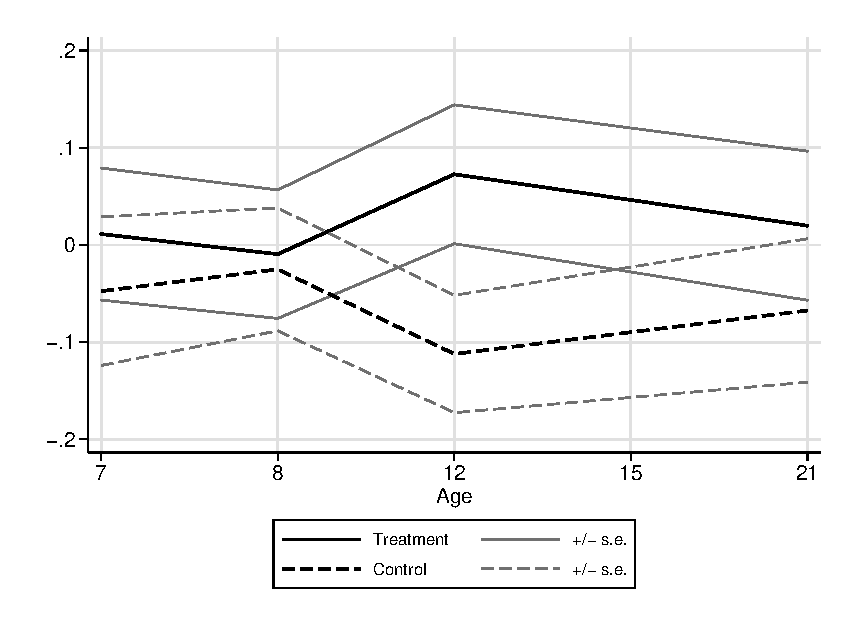
\includegraphics[width=30em]{output/abccareiqranks_0}
\end{center}
\raggedright \footnotesize
Note: This figure shows the growth in the average quantile in IQ with respect to the average quantile at age 5, by treatment and control status. IQ is measured differently across ages (e.g. Stanford-Binet IQ score, Wechsler Preschool and Primary Scale of Intelligence). 
\end{figure}


\begin{figure}[htbp]
\begin{center}
	\caption{Quantile Growth in IQ with Respect to Age 5, Males} \label{fig:iq-rank-male}
	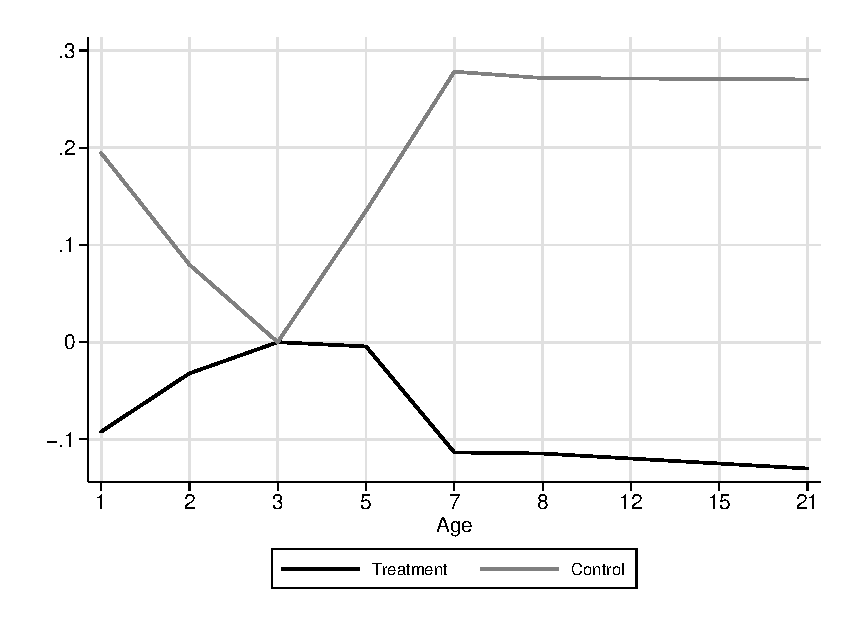
\includegraphics[width=30em]{output/abccareiqranks_1}
\end{center}
\raggedright \footnotesize
Note: This figure shows the growth in the average quantile in IQ with respect to the average quantile at age 5, by treatment and control status. IQ is measured differently across ages (e.g. Stanford-Binet IQ score, Wechsler Preschool and Primary Scale of Intelligence). 
\end{figure}

\section{Alternate Preschool}

We provide some results to show the differential selection by gender into preschool by the families of the control-group children. Overall, we find that females in the control group who went to preschools besides ABC or CARE benefitted more than their male counterparts. This is seen in Table \ref{tab:pq-female} and Table \ref{tab:pq-male}. For both males and females, enrolling in alternative preschool increases the years of education at age 30 by significant amounts, even after accounting for the number of months enrolled. However, for males, the magnitude of the effect is smaller. Furthermore, males are not significantly more likely to be employed at age 30 as a result of enrolling in alternative preschool. The direction of the effect is imprecise and negative.

\begin{table}[htbp]
\begin{center}
	\caption{Age-30 Outcomes and Selection into Preschool, Females} \label{tab:pq-female}
	\scalebox{1}{
		\begin{tabular}{lcccccc} 
\toprule
& \mc{3}{c}{Yrs. of Edu.} & \mc{3}{c}{Employed} \\
\cmidrule(lr){2-4} \cmidrule(lr){5-7}
 & (1) & (2) & (3) & (4) & (5) & (6) \\
 \midrule
 &  &  &  &  &  &  \\
Enrollment indicator & 2.829*** &  & 2.760* & 0.353* &  & 0.552** \\
 & (0.972) &  & (1.374) & (0.183) &  & (0.252) \\
Months enrolled &  & 0.041* & 0.002 &  & 0.002 & -0.006 \\
 &  & (0.021) & (0.028) &  & (0.004) & (0.005) \\
 &  &  &  &  &  &  \\
 \midrule
$N$ & 34 & 34 & 34 & 34 & 34 & 34 \\
 $R^2$ & 0.351 & 0.250 & 0.351 & 0.292 & 0.201 & 0.325 \\ 
\bottomrule
\end{tabular}

	}
\end{center}
\raggedright \footnotesize
Note: This table shows the relationship between selection into preschool of the control group and age-30 outcomes. The outcomes selected are years of education and a variable indicating employment, both important labor market outcomes. Columns (1) and (4) include an indicator for enrollment as a predictor. Columns (2) and (5) include a variable with the number of months of enrollment as a predictor. Columns (3) and (6) include both of these variables as predictors. All regressions include the following control variables: the High-Risk Index score, the number of siblings in the household when the child was born, the child's Apgar score at both 1 and 5 minutes, an indicator for preterm birth, and an indicator for being in the ABC randomization (as opposed to the CARE randomization). Standard errors in parentheses. *** p$<$0.01, ** p$<$0.05, * p$<$0.10.
\end{table}

\begin{table}[htbp]
\begin{center}
	\caption{Age-30 Outcomes and Selection into Preschool, Males} \label{tab:pq-male}
	\scalebox{1}{
		\begin{tabular}{lcccccc} 
\toprule
& \mc{3}{c}{Yrs. of Edu.} & \mc{3}{c}{Employed} \\
\cmidrule(lr){2-4} \cmidrule(lr){5-7}
 & (1) & (2) & (3) & (4) & (5) & (6) \\
\midrule
 &  &  &  &  &  &  \\
Enrollment indicator & 1.763* &  & 2.588* & -0.015 &  & 0.236 \\
 & (0.906) &  & (1.385) & (0.264) &  & (0.402) \\
Months enrolled &  & 0.018 & -0.023 &  & -0.003 & -0.007 \\
 &  & (0.020) & (0.029) &  & (0.006) & (0.009) \\
 &  &  &  &  &  &  \\
 \midrule
$N$ & 29 & 29 & 29 & 29 & 29 & 29 \\
$R^2$ & 0.283 & 0.188 & 0.303 & 0.132 & 0.146 & 0.160 \\ 
 \bottomrule
\end{tabular}

	}
\end{center}
\raggedright \footnotesize
Note: This table shows the relationship between selection into preschool of the control group and age-30 outcomes. The outcomes selected are years of education and a variable indicating employment, both important labor market outcomes. Columns (1) and (4) include an indicator for enrollment as a predictor. Columns (2) and (5) include a variable with the number of months of enrollment as a predictor. Columns (3) and (6) include both of these variables as predictors. All regressions include the following control variables: the High-Risk Index score, the number of siblings in the household when the child was born, the child's Apgar score at both 1 and 5 minutes, an indicator for preterm birth, and an indicator for being in the ABC randomization (as opposed to the CARE randomization). Standard errors in parentheses. *** p$<$0.01, ** p$<$0.05, * p$<$0.10.
\end{table}

%hrabc_index
%hh_sibs0y
%apgar1
%apgar5
%prem_birth
%abc


\end{document}
